\begin{figure}[t]
\centering
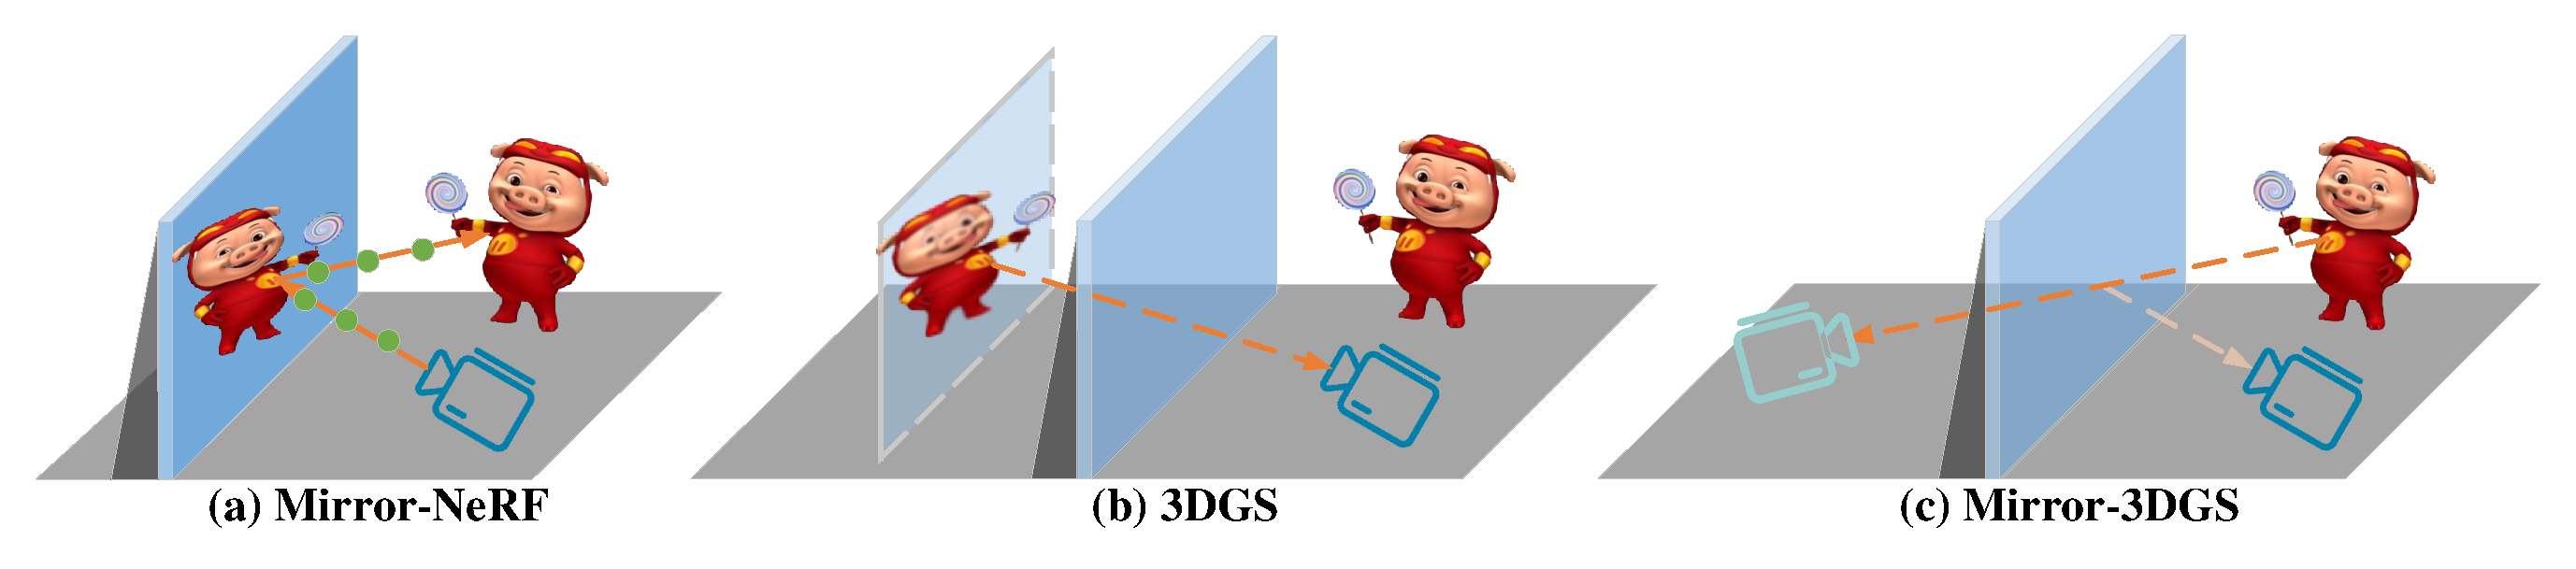
\includegraphics[width=\columnwidth]{file/GGBOND_2.pdf}
\caption{\textbf{The underlying principles in handling mirrored contents}. \textbf{a)} Mirror-NeRF employs a technique involving ray tracing and sampling to achieve mirror reflection. \textbf{b)} 3DGS mistakenly considers objects reflected by the mirror to be placed behind it, resulting the floaters behind the mirror.  \textbf{c)} Our proposed Mirror-3DGS, captures the reflected objects by simulating a novel viewpoint situated behind the mirror.} 
\vskip -0.2in
\label{figure: GGBOND}
\end{figure}